
\vspace{0.15cm}
\begin{flushleft}
	{\color{blue!50!green}\fbox{\fontfamily{qag}\bfseries\selectfont PHẦN I. Câu trắc nghiệm nhiều phương án lựa chọn (3,0 điểm)}}
	\textit{\small (Thí sinh trả lời từ câu 1 đến câu 12. Mỗi câu hỏi thí sinh chỉ chọn một phương án.)}
\end{flushleft}
\setcounter{ex}{0}
\setcounter{bt}{0}

% Câu 1
\begin{ex}
	\macau{ID: VL10-PDL1008-C01}Chuyển động nào sau đây là chuyển động biến đổi?
	\choice
	{Chuyển động thẳng đều}
	{Chuyển động có độ dịch chuyển giảm đều theo thời gian}
	{\True Chuyển động tròn đều}
	{Chuyển động có độ dịch chuyển tăng đều theo thời gian}
	\loigiai{
		Chuyển động tròn đều tuy có tốc độ không đổi nhưng hướng của vectơ vận tốc liên tục thay đổi theo thời gian, do đó là chuyển động biến đổi.\par
	}
\end{ex}

% Câu 2
\begin{ex}
	\macau{ID: VL10-PDL1008-C02}Đối tượng nghiên cứu tổng quát của khoa học Vật lí là
	\choice
	{quy luật tương tác của các dạng năng lượng độc lập}
	{\True các dạng vận động của vật chất và các dạng năng lượng trong tự nhiên}
	{các dạng vận động và tương tác cơ học của vật chất vô cơ}
	{các quy luật nhiệt động lực học ứng dụng}
	\loigiai{
		Vật lí học tập trung nghiên cứu về các dạng vận động cơ bản của vật chất và các dạng năng lượng tương tác giữa chúng trong tự nhiên từ cấp vi mô đến vĩ mô.\par
	}
\end{ex}

% Câu 3
\begin{ex}
	\macau{ID: VL10-PDL1008-C03}Một người đi xe máy từ nhà đến bến xe buýt cách nhà $6\text{ km}$ về phía Đông, sau đó lên xe buýt đi tiếp $6\text{ km}$ thẳng về phía Bắc. Độ lớn độ dịch chuyển tổng hợp của người này là
	\choice
	{$6\text{ km}$}
	{$12\text{ km}$}
	{$72\text{ km}$}
	{\True $6\sqrt{2}\text{ km}$}
	\loigiai{
		Hai hướng chuyển động Đông và Bắc vuông góc với nhau.\par
		Độ lớn độ dịch chuyển tổng hợp:\par
		\[d = \sqrt{d_1^2 + d_2^2} = \sqrt{6^2 + 6^2} = 6\sqrt{2}\text{ km}.\]
	}
\end{ex}

% Câu 4
\begin{ex}
	\macau{ID: VL10-PDL1008-C04}Hành động nào sau đây \textbf{không} thuộc về phương pháp lí thuyết trong nghiên cứu Vật lí?
	\choice
	{\True Thực hiện ném một quả bóng lên cao để quan sát quá trình chuyển động rơi}
	{Chế tạo quả địa cầu làm mô hình thu nhỏ của Trái Đất}
	{Biểu diễn đường truyền của chùm sáng bằng các tia sáng hình học}
	{Tính toán quỹ đạo chuyển động của các hành tinh dựa trên phương trình toán học}
	\loigiai{
		Hành động ném quả bóng để quan sát chuyển động thuộc về phương pháp thực nghiệm, không phải phương pháp lí thuyết hay mô hình hóa.\par
	}
\end{ex}

% Câu 5
\begin{ex}
	\macau{ID: VL10-PDL1008-C05}Phát biểu nào sau đây \textbf{sai} khi nói về các cuộc cách mạng công nghiệp trong lịch sử?
	\choice
	{Với cuộc cách mạng công nghiệp lần thứ hai, con người đã sản xuất được điện năng và đưa vào phục vụ sản xuất, đời sống}
	{Internet kết nối vạn vật, trí tuệ nhân tạo và công nghệ nano là các đặc trưng tiêu biểu của cách mạng công nghiệp lần thứ tư}
	{\True Đặc trưng cốt lõi của cuộc cách mạng công nghiệp lần thứ ba là thay thế sức cơ bắp của con người bằng máy móc cơ khí cơ bản}
	{Động cơ hơi nước do James Watt cải tiến năm 1769 là dấu mốc mở đầu cuộc cách mạng công nghiệp lần thứ nhất}
	\loigiai{
		Việc thay thế sức cơ bắp bằng máy móc cơ khí chạy bằng hơi nước là đặc trưng cốt lõi của cuộc cách mạng công nghiệp lần thứ nhất. Cách mạng công nghiệp lần thứ ba đặc trưng bởi tự động hóa và công nghệ thông tin.\par
	}
\end{ex}

% Câu 6
\begin{ex}
	\macau{ID: VL10-PDL1008-C06}Phát biểu nào sau đây đúng khi nói về bản chất của đại lượng vận tốc tức thời?
	\choice
	{\True Là đại lượng vectơ, cho biết mức độ nhanh chậm và hướng chuyển động của vật}
	{Là đại lượng vô hướng, cho biết tổng thời gian chuyển động của vật}
	{Là đại lượng vectơ, cho biết thời gian và quãng đường chuyển động của vật}
	{Là đại lượng vô hướng, chỉ cho biết mức độ nhanh chậm đơn thuần của chuyển động}
	\loigiai{
		Vận tốc tức thời $\vec{v}$ là đại lượng vectơ, có độ lớn cho biết mức độ nhanh chậm và có hướng cho biết hướng chuyển động của vật tại thời điểm xét.\par
	}
\end{ex}

% Câu 7
\begin{ex}
	\macau{ID: VL10-PDL1008-C07}Một học sinh thực hành đo tốc độ của viên bi thép thu được kết quả: $v = 2{,}5 \pm 0{,}02\text{ (m/s)}$. Sai số tỉ đối $\delta v$ của phép đo này bằng
	\choice
	{$0{,}2\%$}
	{$4{,}0\%$}
	{\True $0{,}8\%$}
	{$1{,}6\%$}
	\loigiai{
		Sai số tỉ đối của phép đo:\par
		\[\delta v = \frac{\Delta v}{\overline{v}} \cdot 100\% = \frac{0{,}02}{2{,}5} \cdot 100\% = 0{,}8\%.\]
	}
\end{ex}

% Câu 8
\begin{ex}
	\macau{ID: VL10-PDL1008-C08}Độ dịch chuyển là một đại lượng vectơ cho biết
	\choice
	{\True độ dài và hướng của sự thay đổi vị trí của vật}
	{tọa độ và hướng chuyển động tức thời của vật}
	{tổng chiều dài quãng đường thực tế mà vật đã đi được}
	{tốc độ trung bình trên toàn bộ hành trình của vật}
	\loigiai{
		Độ dịch chuyển $\vec{d}$ là vectơ nối vị trí đầu và vị trí cuối của vật, cho biết độ dài và hướng của sự thay đổi vị trí của vật.\par
	}
\end{ex}

% Câu 9
\begin{ex}
	\macau{ID: VL10-PDL1008-C09}Ưu điểm nổi bật nhất của thiết bị cổng quang điện kết hợp với đồng hồ đo thời gian hiện số so với đồng hồ bấm giây cơ học là
	\choice
	{có thể tự động đo được tất cả các đại lượng vật lí}
	{luôn cho kết quả đo nhanh nhất trong mọi tình huống}
	{\True loại bỏ được sai số chủ quan của con người khi bấm nút và có độ chính xác rất cao}
	{thiết bị có cấu tạo thô sơ và giá thành rẻ hơn}
	\loigiai{
		Cổng quang điện tự động kích hoạt và ngắt tín hiệu khi vật chắn chùm sáng, loại bỏ hoàn toàn sai số phản xạ chủ quan của người bấm đồng hồ cơ học, đem lại độ chính xác cao.\par
	}
\end{ex}

% Câu 10
\begin{ex}
	\macau{ID: VL10-PDL1008-C10}Chọn phát biểu \textbf{không} đúng về các quy tắc an toàn trong phòng thực hành Vật lí.
	\choice
	{Chọn sai thang đo khi dùng đồng hồ đo điện có thể làm hỏng hoặc chập cháy thiết bị}
	{\True Chỉ cần sử dụng thiết bị đo có lớp vỏ bằng nhựa hoặc kim loại thì sẽ tuyệt đối an toàn}
	{Đun nóng hóa chất dễ cháy bằng thiết bị điện công suất lớn có thể dẫn đến nguy cơ hỏa hoạn}
	{Thao tác sai quy trình kĩ thuật có thể dẫn đến tai nạn, chấn thương cho người làm thí nghiệm}
	\loigiai{
		Vỏ cách điện chỉ là biện pháp bảo vệ cơ bản, việc đảm bảo an toàn tuyệt đối phụ thuộc vào việc tuân thủ đúng quy trình kĩ thuật và quy tắc an toàn khi vận hành nguồn điện.\par
	}
\end{ex}

% Câu 11
\begin{ex}
	\macau{ID: VL10-PDL1008-C11}Khi phát hiện sự cố chập điện gây cháy trong phòng thực hành Vật lí, thứ tự các hành động xử lí đúng là
	\choice
	{dùng nước dội trực tiếp ngay vào đám cháy}
	{\True ngắt ngay cầu dao điện toàn khu, sơ tán vật dễ cháy ra xa, cứu người và tài sản, dập tắt đám cháy bằng bình chuyên dụng}
	{hô hoán rồi chạy nhanh ra ngoài mà không làm gì thêm}
	{chỉ ngắt nguồn điện rồi dùng nước dội vào đám cháy}
	\loigiai{
		Phải ngắt ngay nguồn điện trước tiên để tránh nguy cơ điện giật và chập cháy lan, sau đó sơ tán chất dễ cháy, cứu hộ và dập lửa bằng bình chữa cháy thích hợp (như bình bột hoặc bình khí $\text{CO}_2$).\par
	}
\end{ex}

% Câu 12
\begin{ex}
	\macau{ID: VL10-PDL1008-C12}Gọi $\overline{A}$ là giá trị trung bình và $\Delta A$ là sai số tuyệt đối toàn phần của phép đo đại lượng $A$. Sai số tỉ đối $\delta A$ được xác định theo công thức nào?
	\choice
	{\True $\delta A = \dfrac{\Delta A}{\overline{A}} \cdot 100\%$}
	{$\delta A = \dfrac{\overline{A}}{\Delta A} \cdot 100\%$}
	{$\delta A = \Delta A \cdot \overline{A} \cdot 100\%$}
	{$\delta A = \dfrac{\Delta A}{\overline{A}}$}
	\loigiai{
		Sai số tỉ đối $\delta A$ là tỉ số phần trăm giữa sai số tuyệt đối và giá trị trung bình: $\delta A = \dfrac{\Delta A}{\overline{A}} \cdot 100\%$.\par
	}
\end{ex}

\vspace{0.15cm}
\begin{flushleft}
	{\color{blue!50!green}\fbox{\fontfamily{qag}\bfseries\selectfont PHẦN II. Câu trắc nghiệm đúng sai (2,0 điểm)}}
	\textit{\small (Thí sinh trả lời từ câu 1 đến câu 2. Trong mỗi ý a), b), c), d) ở mỗi câu, thí sinh chọn đúng hoặc sai.)}
\end{flushleft}
\setcounter{ex}{0}
\setcounter{bt}{0}

% Phần II Câu 1
\begin{ex}
	\macau{ID: VL10-PDL1008-C13}Một học sinh dùng panme có sai số dụng cụ $0{,}01\text{ mm}$ để đo đường kính $d$ của một viên bi thép nhỏ. Kết quả qua 5 lần đo được ghi trong bảng sau:
	\choiceTF[t]
	{\True Muốn đánh giá mức độ chính xác của phép đo, ta căn cứ vào giá trị sai số tỉ đối của phép đo đó.}
	{Bán kính trung bình của viên bi thép thu được từ chuỗi phép đo bằng $6{,}49\text{ mm}$.}
	{\True Kết quả phép đo đường kính kèm sai số toàn phần được viết là $d = 6{,}49 \pm 0{,}03\text{ (mm)}$.}
	{Phương pháp dùng panme để xác định trực tiếp đường kính viên bi là một phép đo gián tiếp.}
	\loigiai{
		{\color{green!50!black}\textbf{a) Đúng.}} Sai số tỉ đối phản ánh mức độ chính xác của phép đo: sai số tỉ đối càng nhỏ thì phép đo càng chính xác.\par
		{\color{red!80!black}\textbf{b) Sai.}} Giá trị trung bình từ bảng là đường kính trung bình: $\overline{d} = \dfrac{6{,}47 + 6{,}48 + 6{,}51 + 6{,}47 + 6{,}52}{5} = 6{,}49\text{ mm}$, không phải bán kính.\par
		{\color{green!50!black}\textbf{c) Đúng.}} Sai số ngẫu nhiên: $\overline{\Delta d} = \dfrac{0{,}02 + 0{,}01 + 0{,}02 + 0{,}02 + 0{,}03}{5} = 0{,}02\text{ mm}$. Sai số toàn phần: $\Delta d = \overline{\Delta d} + \Delta d_{\text{dc}} = 0{,}02 + 0{,}01 = 0{,}03\text{ mm}$. Kết quả đúng: $d = 6{,}49 \pm 0{,}03\text{ mm}$.\par
		{\color{red!80!black}\textbf{d) Sai.}} Đường kính viên bi được đọc trực tiếp từ thang chia của panme nên đây là phép đo trực tiếp.\par
	}
\end{ex}

% Phần II Câu 2
\begin{ex}
	\macau{ID: VL10-PDL1008-C14}Một vật bắt đầu chuyển động thẳng nhanh dần đều trên phương ngang từ trạng thái nghỉ ($v_0 = 0$). Sau khi đi được quãng đường $100\text{ m}$ đầu tiên, vật đạt tốc độ $20\text{ m/s}$. Chọn chiều dương là chiều chuyển động của vật.
	\choiceTF[t]
	{Trong hệ SI, đơn vị đo tiêu chuẩn của gia tốc là mét trên giây ($\text{m/s}$).}
	{Vận tốc tức thời của vật sau thời gian $t = 5\text{ s}$ kể từ lúc xuất phát bằng $15\text{ m/s}$.}
	{\True Vì vật chuyển động nhanh dần đều nên gia tốc $a$ và vận tốc tức thời $v$ luôn cùng dấu đại số.}
	{Gia tốc của chuyển động này có giá trị đại số là $a = -2\text{ m/s}^2$.}
	\loigiai{
		{\color{red!80!black}\textbf{a) Sai.}} Đơn vị tiêu chuẩn của gia tốc trong hệ SI là mét trên giây bình phương ($\text{m/s}^2$).\par
		{\color{red!80!black}\textbf{b) Sai.}} Áp dụng hệ thức: $v^2 - v_0^2 = 2as \Rightarrow 20^2 - 0 = 2 \cdot a \cdot 100 \Rightarrow a = 2\text{ m/s}^2$. Sau $5\text{ s}$: $v = at = 2 \cdot 5 = 10\text{ m/s} \ne 15\text{ m/s}$.\par
		{\color{green!50!black}\textbf{c) Đúng.}} Chuyển động thẳng nhanh dần đều có $a \cdot v > 0$ nên $a$ và $v$ luôn cùng dấu.\par
		{\color{red!80!black}\textbf{d) Sai.}} Vật chuyển động nhanh dần theo chiều dương nên gia tốc có giá trị dương: $a = +2\text{ m/s}^2$.\par
	}
\end{ex}

\vspace{0.15cm}
\begin{flushleft}
	{\color{blue!50!green}\fbox{\fontfamily{qag}\bfseries\selectfont PHẦN III. Câu trắc nghiệm trả lời ngắn (2,0 điểm)}}
	\textit{\small (Thí sinh trả lời từ câu 1 đến câu 4.)}
\end{flushleft}
\setcounter{ex}{0}
\setcounter{bt}{0}

% Phần III Câu 1
\begin{ex}
	\macau{ID: VL10-PDL1008-C15}Trong một đợt cứu hộ lũ lụt, ca nô chạy xuôi dòng nước với tốc độ $8\text{ m/s}$ so với dòng nước. Vận tốc dòng nước chảy đối với bờ sông là $4\text{ m/s}$. Khoảng cách từ trạm xuất phát đến vị trí người cần cứu nạn là $3\text{ km}$. Tính thời gian (theo đơn vị giây) để ca nô tiếp cận vị trí người cần cứu nạn?

	\par\shortans[oly]{250}
	\loigiai{
		Đổi khoảng cách: $s = 3\text{ km} = 3000\text{ m}$.\par
		Vận tốc của ca nô đối với bờ khi xuôi dòng:\par
		\[v = v_{\text{cn/n}} + v_{\text{n/b}} = 8 + 4 = 12\text{ m/s}.\]
		Thời gian chuyển động của ca nô:\par
		\[t = \frac{s}{v} = \frac{3000}{12} = 250\text{ s}.\]
	}
\end{ex}

% Phần III Câu 2
\begin{ex}
	\macau{ID: VL10-PDL1008-C16}Một ô tô đứng yên bắt đầu chuyển động thẳng nhanh dần đều từ trạng thái nghỉ. Trong giây thứ 5 kể từ lúc xuất phát, xe đi được quãng đường $13{,}5\text{ m}$. Gia tốc của ô tô bằng bao nhiêu $\text{m/s}^2$?

	\par\shortans[oly]{3}
	\loigiai{
		Quãng đường ô tô đi được trong giây thứ 5:\par
		\[\Delta s_5 = s(5) - s(4) = \frac{1}{2}a \cdot 5^2 - \frac{1}{2}a \cdot 4^2 = \frac{9}{2}a = 4{,}5a\text{ (m)}.\]
		Thay $\Delta s_5 = 13{,}5\text{ m}$:\par
		\[13{,}5 = 4{,}5a \Rightarrow a = 3\text{ m/s}^2.\]
	}
\end{ex}

% Phần III Câu 3
\begin{ex}
	\macau{ID: VL10-PDL1008-C17}Một ô tô chuyển động thẳng đều có đồ thị độ dịch chuyển -- thời gian $(d - t)$ là đường thẳng đi qua gốc tọa độ $O$. Tại thời điểm $t = 2\text{ h}$, độ dịch chuyển của xe là $80\text{ km}$. Vận tốc của ô tô bằng bao nhiêu $\text{km/h}$?

	\par\shortans[oly]{40}
	\loigiai{
		Vận tốc của chuyển động thẳng đều:\par
		\[v = \frac{d}{t} = \frac{80}{2} = 40\text{ km/h}.\]
	}
\end{ex}

% Phần III Câu 4
\begin{ex}
	\macau{ID: VL10-PDL1008-C18}Một xe máy chuyển động thẳng nhanh dần đều từ trạng thái nghỉ ($v_0 = 0$). Sau khi đi được quãng đường $100\text{ m}$ đầu tiên, xe đạt vận tốc $10\text{ m/s}$. Vận tốc của xe sau khi đi thêm được quãng đường $100\text{ m}$ tiếp theo là bao nhiêu $\text{m/s}$? (Làm tròn kết quả đến một chữ số thập phân).

	\par\shortans[oly]{14,1}
	\loigiai{
		Gia tốc của xe trên $100\text{ m}$ đầu:\par
		\[v_1^2 - v_0^2 = 2as_1 \Rightarrow 10^2 - 0 = 2 \cdot a \cdot 100 \Rightarrow a = 0{,}5\text{ m/s}^2.\]
		Tổng quãng đường xe đi được sau hai chặng: $S = s_1 + s_2 = 100 + 100 = 200\text{ m}$.\par
		Vận tốc tại thời điểm đó:\par
		\[v_2^2 - v_0^2 = 2aS \Rightarrow v_2 = \sqrt{2 \cdot 0{,}5 \cdot 200} = \sqrt{200} = 10\sqrt{2} \approx 14{,}1\text{ m/s}.\]
	}
\end{ex}

\vspace{0.15cm}
\begin{flushleft}
	{\color{blue!50!green}\fbox{\fontfamily{qag}\bfseries\selectfont PHẦN IV. Tự luận (3,0 điểm)}}
	\textit{\small (Thí sinh trình bày lời giải từ câu 1 đến câu 2.)}
\end{flushleft}
\setcounter{ex}{0}
\setcounter{bt}{0}

% Phần IV Câu 1
\begin{ex}
	\macau{ID: VL10-PDL1008-C19}Một vận động viên bơi ngang từ bờ sông bên này sang bờ bên kia theo phương vuông góc với dòng sông rộng $50\text{ m}$ (hướng từ Tây sang Đông). Nước sông chảy theo hướng từ Bắc xuống Nam khiến người đó bị cuốn trôi xuôi về phía hạ lưu một đoạn $50\text{ m}$.
	\par \textbf{a)} Vẽ hình minh họa và xác định hướng của vectơ độ dịch chuyển tổng hợp của người đó. \par \textbf{b)} Tính độ lớn của độ dịch chuyển tổng hợp.
	\begin{center}
		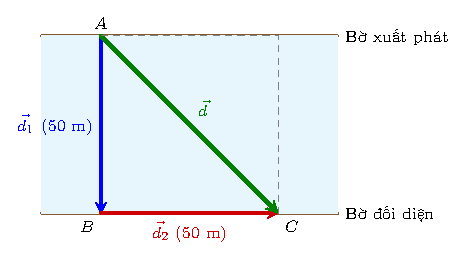
\includegraphics[width=7.0cm]{fig_nguoi_boi.pdf}
	\end{center}
	\loigiai{
		\textbf{a)} Minh họa chuyển động:\par
		-- Chọn gốc $A$ tại vị trí xuất phát ở bờ bên này. Vectơ $\vec{d}_1 = \vec{AB}$ hướng sang bờ đối diện biểu diễn độ rộng dòng sông ($AB = 50\text{ m}$).\par
		-- Vectơ $\vec{d}_2 = \vec{BC}$ hướng theo dòng nước chảy dọc bờ sông ($BC = 50\text{ m}$).\par
		-- Vectơ độ dịch chuyển tổng hợp là $\vec{d} = \vec{AC} = \vec{d}_1 + \vec{d}_2$. Vectơ này có hướng Đông -- Nam, lệch góc $45^\circ$ so với phương bơi ban đầu.\par
		\textbf{b)} Do $\vec{d}_1 \perp \vec{d}_2$, áp dụng định lí Pythagore:\par
		\[d = AC = \sqrt{AB^2 + BC^2} = \sqrt{50^2 + 50^2} = 50\sqrt{2} \approx 70{,}71\text{ m}.\]
	}
\end{ex}

% Phần IV Câu 2
\begin{ex}
	\macau{ID: VL10-PDL1008-C20}Một chất điểm chuyển động thẳng dọc theo trục $Ox$ có đồ thị vận tốc -- thời gian $(v - t)$ như hình bên.
	\par \textbf{a)} Tính độ biến thiên vận tốc $\Delta v$ của chất điểm từ thời điểm $t = 0$ đến thời điểm $t = 20\text{ s}$. \par \textbf{b)} Tính gia tốc $a$ của chất điểm trong giai đoạn $CD$ (từ $t = 40\text{ s}$ đến $t = 80\text{ s}$).
	\begin{center}
		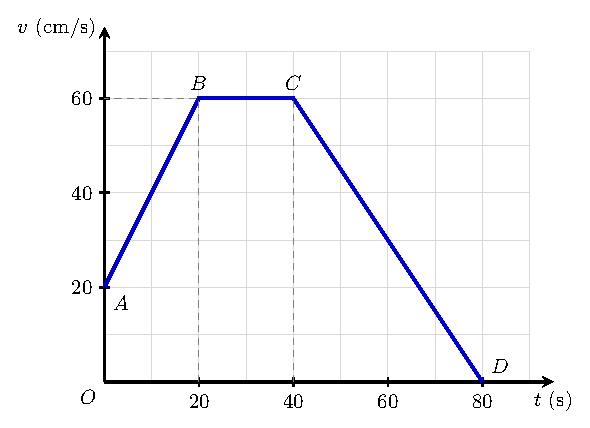
\includegraphics[width=7.5cm]{fig_dothi_vt.pdf}
	\end{center}
	\loigiai{
		\textbf{a)} Từ đồ thị, tại thời điểm $t = 0$ có $v_A = 20\text{ cm/s}$; tại thời điểm $t = 20\text{ s}$ có $v_B = 60\text{ cm/s}$.\par
		Độ biến thiên vận tốc trong giai đoạn $AB$:\par
		\[\Delta v = v_B - v_A = 60 - 20 = 40\text{ cm/s} = 0{,}4\text{ m/s}.\]
		\textbf{b)} Trong giai đoạn $CD$, tại $t_C = 40\text{ s}$ có $v_C = 60\text{ cm/s}$; tại $t_D = 80\text{ s}$ có $v_D = 0$.\par
		Gia tốc của chất điểm trên đoạn $CD$:\par
		\[a_{CD} = \frac{v_D - v_C}{t_D - t_C} = \frac{0 - 60}{80 - 40} = -1{,}5\text{ cm/s}^2 = -0{,}015\text{ m/s}^2.\]
	}
\end{ex}
